\chapter{Introducción}
En esta práctica, vamos a trabajar con una máquina de Turing diseñada para reconocer el lenguaje {$0^n$$1^n$ | n >=1}, es decir, cadenas formadas por una secuencia de ceros seguida por una secuencia de unos, donde el número de ceros y unos es el mismo y mayor o igual a uno. Esta máquina de Turing se basa en el libro de John Hopcroft, en el ejercicio 8.2 de la segunda edición.\newline

La máquina de Turing que construiremos seguirá un proceso específico para transformar la entrada dada. Comenzando desde el extremo izquierdo de la cinta, la máquina cambiará secuencialmente los ceros por la letra X y se moverá hacia la derecha, pasando por encima de cualquier cero o letra Y que encuentre, hasta que encuentre un uno. En ese momento, cambiará el uno por la letra Y y se moverá hacia la izquierda, pasando sobre cualquier letra Y o cero hasta que encuentre una X. En esta situación, buscará un cero colocado inmediatamente a la derecha y, si lo encuentra, lo cambiará por una X y repetirá el proceso, cambiando el uno correspondiente por una Y.\newline

Si la entrada no cumple con el patrón $0^n$$1^n$, la máquina de Turing se detendrá sin aceptar la cadena. Sin embargo, si la máquina logra cambiar todos los ceros por X en la misma iteración en la que cambia el último uno por una Y, entonces se determina que la entrada es de la forma $0^n$$1^n$ y la máquina la acepta.\newline

En esta práctica, implementaremos la máquina de Turing en Python, permitiendo que el usuario ingrese una cadena o generando una automáticamente. El programa generará un archivo de texto como salida, que contendrá las descripciones instantáneas en cada paso de la computación. También animaremos la máquina de Turing para cadenas de longitud menor o igual a 10 caracteres.\newline

A continuación, se presenta el código de la máquina de Turing y se proporciona en el reporte, junto con el archivo fuente del código.\newline

Esta práctica se basa en conceptos de teoría de la computación, específicamente en el estudio de gramáticas formales y sus derivaciones. El propósito es aplicar estos conceptos para implementar un programa que pueda procesar y generar cadenas válidas según una gramática específica.\newline

La tabla de transiciones a utilizar en el desarrollo de esta práctica es:\newline

\begin{figure}[h]
%\begin{minipage}{0.3\textwidth}
    \begin{center}
    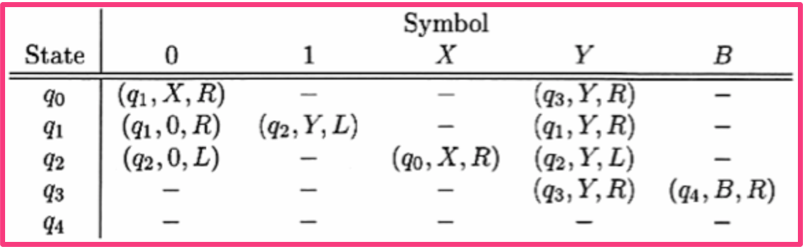
\includegraphics[width=1\linewidth]{Images/tabla.png}
    \end{center}
%\end{minipage}
\caption{Tabla de estados para el problema.}
\label{fig:imagen}
\end{figure}